\documentclass{homework}
\begin{document}
\hwtitle{数值分析上机作业一}{杨弦昊-2023P8270108012}{中国机械总院}
\timu{求$f(x)=\sin(\pi x)$在区间$\left[0,1\right]$上的二次最佳平方逼近多项式$P^{*}(x)$,并绘出$f(x)$和$P^{*}(x)$的图像进行比较。}
\jie
% \begin{equation}
%     \begin{bmatrix}
%         1&\frac{1}{2}&\frac{1}{3}\\
%         \frac{1}{2}&\frac{1}{3}&\frac{1}{4}\\
%         \frac{1}{3}&\frac{1}{4}&\frac{1}{5}\\
%     \end{bmatrix}
%     \begin{bmatrix}
%         c_0\\c_1\\c_2
%     \end{bmatrix}=
%     \begin{bmatrix}
%         \frac{2}{\pi}\\\frac{1}{\pi}\\\frac{1}{pi^2}
%     \end{bmatrix}
% \end{equation}
取空间$\varPhi=\mathrm{Span}\{1,x,x^2\}$,权$\omega(x)=1$,按式\ref{dingjifen}分别计算并存进数组$A[3][3]$、$B[3]$。
\begin{equation}
    \label{dingjifen}
    \left\{
        \begin{aligned}
            (\varphi_i,\varphi_j)&=\int_a^bx^{i+j}\mathrm{d}x,\\
            (f,\varphi_j)&=\int_a^bf(x)x^j\mathrm{d}x
        \end{aligned}
    \right.
\end{equation}
\begin{equation}
    \begin{aligned}
        (\varphi_0,\varphi_0)=A[0][0],\quad&(\varphi_1,\varphi_0)=A[0][1],&(\varphi_2,\varphi_0)=A[0][2],\quad&(f,\varphi_0)=B[0]\\
                            &(\varphi_1,\varphi_1)=A[1][1],&(\varphi_2,\varphi_1)=A[1][2],\quad&(f,\varphi_1)=B[1]\\
                            &&(\varphi_2,\varphi_2)=A[2][2],\quad&(f,\varphi_2)=B[2]
    \end{aligned}
\end{equation}

则正规方程为
\begin{equation}
    \left\{
        \begin{aligned}
            A[0][0]C_0+A[0][1]C_1+A[0][2]C_2&=B[0]\\
            A[1][0]C_0+A[1][1]C_1+A[1][2]C_2&=B[1]\\
            A[2][0]C_0+A[2][1]C_1+A[2][2]C_2&=B[2]\\
        \end{aligned}
    \right.
\end{equation}

解上述线性方程即得二次最佳平方逼近多项式$P^*(x)=C_0+C_1x+C_2x^2$。

通过编写C语言程序即可得到$f(x)=\sin(\pi x)$在区间$\left[0,1\right]$上的二次最佳平方逼近多项式$P^{*}(x)=-4.12251x^2+4.12251x-0.050465$;$f(x)$和$P^{*}(x)$的图像如图\ref{answer1}所示;代码如下:
\begin{figure}[htbp]
    \centering
    \includegraphics[width=.9\linewidth]{figure/answer1.pdf}
    \caption{$f(x)$和$P^{*}(x)$的图像}
    \label{answer1}
\end{figure}
\lstinputlisting{code/answer1.c}
\clearpage
\timu{对Runge函数$R(x)$(式(2.5.2)),利用下列条件作插值逼近,并与$R(x)$的图像进行比较。

(1)用等距节点$x_i=-5+i(i=0,1,2,\cdots,10)$,绘出它的10次Newton插值多项式的图像;

(2)用节点$x_i=5\cos\left(\frac{2i+1}{42}\pi\right)(i=0,1,2,\cdots,20)$,绘出它的20次Lagrange插值多项式的图像;

(3)用等距节点$x_i=-5+i(i=0,1,2,\cdots,10)$,绘出它的分段线性插值函数的图像;

(4)用等距节点$x_i=-5+i(i=0,1,2,\cdots,10)$,绘出它的分段三次Hermite插值函数图像;

(5)用等距节点$x_i=-5+i(i=0,1,2,\cdots,10)$,绘出它的三次自然样条插值函数的图像。}
\jie

(1)如图\ref{newton}所示,可以看到Newton插值多项式图像在中部与$R(x)$拟合程度较好,而在两端由于计算的舍入误差会迅速扩大,因此图像产生较大波动。
\begin{figure}[htbp]
    \centering
    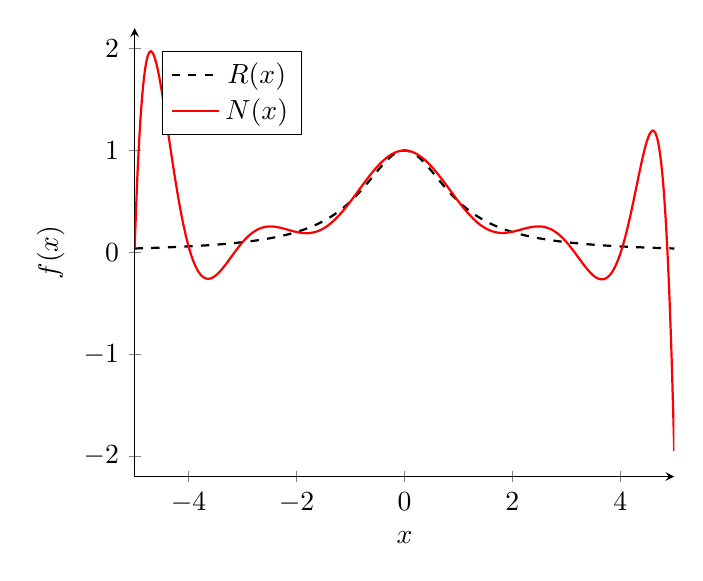
\begin{tikzpicture}
        % 绘制函数 1 / (1 + x^2)
        \begin{axis}[
            axis lines = left,
            xlabel = $x$,
            ylabel = $f(x)$,
            xmin = -5,
            xmax = 5,
            ymin = -2.2,
            ymax = 2.2,
            legend pos = north west,
            legend style={at={(0.05,0.95)},anchor=north west},
        ]
        \addplot[domain=-5:5, samples=200, black, thick,dashed] {1 / (1 + x^2)};
        \addlegendentry{$R(x)$};
        %\addlegendentry{$\frac{1}{1+x^2}$}
        
        % 绘制插值多项式
        \addplot[color=red, domain=-5:5, samples=200,thick,smooth] {0.038462+(x+5.0)*0.020362+(x+5.0)*(x+4.0)*0.010407+(x+5.0)*(x+4.0)*(x+3.0)*0.006335+(x+5.0)*(x+4.0)*(x+3.0)*(x+2.0)*0.004299+(x+5.0)*(x+4.0)*(x+3.0)*(x+2.0)*(x+1.0)*-0.002036+(x+5.0)*(x+4.0)*(x+3.0)*(x+2.0)*(x+1.0)*(x+-0.0)*-0.001131+(x+5.0)*(x+4.0)*(x+3.0)*(x+2.0)*(x+1.0)*(x+-0.0)*(x+-1.0)*0.001086+(x+5.0)*(x+4.0)*(x+3.0)*(x+2.0)*(x+1.0)*(x+-0.0)*(x+-1.0)*(x+-2.0)*-0.000430+(x+5.0)*(x+4.0)*(x+3.0)*(x+2.0)*(x+1.0)*(x+-0.0)*(x+-1.0)*(x+-2.0)*(x+-3.0)*0.000113+(x+5.0)*(x+4.0)*(x+3.0)*(x+2.0)*(x+1.0)*(x+-0.0)*(x+-1.0)*(x+-2.0)*(x+-3.0)*(x+-4.0)*-0.000023};
        \addlegendentry{$N(x)$}
        \end{axis}
        \end{tikzpicture}
    \caption{$R(x)$图像与$N(x)$图像}
    \label{newton}
\end{figure}

代码如下:
\lstinputlisting{code/answer2-1.c}
\clearpage
(2)如图\ref{lagrange}所示,与Newton插值类似,Lagrange插值也会在两端产生波动。
\begin{figure}[htbp]
    \centering
    \begin{tikzpicture}
        % 绘制函数 1 / (1 + x^2)
        \begin{axis}[
            axis lines = left,
            xlabel = $x$,
            ylabel = $f(x)$,
            xmin = -5,
            xmax = 5,
            ymin = -0.2,
            ymax = 1.2,
            legend pos = north west,
            legend style={at={(0.05,0.95)},anchor=north west},
        ]
        \addplot[domain=-5:5, samples=200, black, thick,dashed] {1 / (1 + x^2)};
        \addlegendentry{$R(x)$}
        
        % 绘制插值多项式
        \addplot[domain=-5:5, red, thick,samples=200,smooth] {(0.038669)*((x-4.874640)*(x-4.654369)*(x-4.330127)*(x-3.909157)*(x-3.400864)*(x-2.816600)*(x-2.169419)*(x-1.473776)*(x-0.745211)*(x-0.000000)*(x--0.745211)*(x--1.473776)*(x--2.169419)*(x--2.816600)*(x--3.400864)*(x--3.909157)*(x--4.330127)*(x--4.654369)*(x--4.874640)*(x--4.986019)/(25557827938.677975))+(0.040384)*((x-4.986019)*(x-4.654369)*(x-4.330127)*(x-3.909157)*(x-3.400864)*(x-2.816600)*(x-2.169419)*(x-1.473776)*(x-0.745211)*(x-0.000000)*(x--0.745211)*(x--1.473776)*(x--2.169419)*(x--2.816600)*(x--3.400864)*(x--3.909157)*(x--4.330127)*(x--4.654369)*(x--4.874640)*(x--4.986019)/(-8583187387.206031))+(0.044124)*((x-4.986019)*(x-4.874640)*(x-4.330127)*(x-3.909157)*(x-3.400864)*(x-2.816600)*(x-2.169419)*(x-1.473776)*(x-0.745211)*(x-0.000000)*(x--0.745211)*(x--1.473776)*(x--2.169419)*(x--2.816600)*(x--3.400864)*(x--3.909157)*(x--4.330127)*(x--4.654369)*(x--4.874640)*(x--4.986019)/(5227824816.650484))+(0.050633)*((x-4.986019)*(x-4.874640)*(x-4.654369)*(x-3.909157)*(x-3.400864)*(x-2.816600)*(x-2.169419)*(x-1.473776)*(x-0.745211)*(x-0.000000)*(x--0.745211)*(x--1.473776)*(x--2.169419)*(x--2.816600)*(x--3.400864)*(x--3.909157)*(x--4.330127)*(x--4.654369)*(x--4.874640)*(x--4.986019)/(-3819877747.446303))+(0.061419)*((x-4.986019)*(x-4.874640)*(x-4.654369)*(x-4.330127)*(x-3.400864)*(x-2.816600)*(x-2.169419)*(x-1.473776)*(x-0.745211)*(x-0.000000)*(x--0.745211)*(x--1.473776)*(x--2.169419)*(x--2.816600)*(x--3.400864)*(x--3.909157)*(x--4.330127)*(x--4.654369)*(x--4.874640)*(x--4.986019)/(3063304111.838376))+(0.079581)*((x-4.986019)*(x-4.874640)*(x-4.654369)*(x-4.330127)*(x-3.909157)*(x-2.816600)*(x-2.169419)*(x-1.473776)*(x-0.745211)*(x-0.000000)*(x--0.745211)*(x--1.473776)*(x--2.169419)*(x--2.816600)*(x--3.400864)*(x--3.909157)*(x--4.330127)*(x--4.654369)*(x--4.874640)*(x--4.986019)/(-2605462105.915654))+(0.111942)*((x-4.986019)*(x-4.874640)*(x-4.654369)*(x-4.330127)*(x-3.909157)*(x-3.400864)*(x-2.169419)*(x-1.473776)*(x-0.745211)*(x-0.000000)*(x--0.745211)*(x--1.473776)*(x--2.169419)*(x--2.816600)*(x--3.400864)*(x--3.909157)*(x--4.330127)*(x--4.654369)*(x--4.874640)*(x--4.986019)/(2311606442.464890))+(0.175243)*((x-4.986019)*(x-4.874640)*(x-4.654369)*(x-4.330127)*(x-3.909157)*(x-3.400864)*(x-2.816600)*(x-1.473776)*(x-0.745211)*(x-0.000000)*(x--0.745211)*(x--1.473776)*(x--2.169419)*(x--2.816600)*(x--3.400864)*(x--3.909157)*(x--4.330127)*(x--4.654369)*(x--4.874640)*(x--4.986019)/(-2119872219.524911))+(0.315257)*((x-4.986019)*(x-4.874640)*(x-4.654369)*(x-4.330127)*(x-3.909157)*(x-3.400864)*(x-2.816600)*(x-2.169419)*(x-0.745211)*(x-0.000000)*(x--0.745211)*(x--1.473776)*(x--2.169419)*(x--2.816600)*(x--3.400864)*(x--3.909157)*(x--4.330127)*(x--4.654369)*(x--4.874640)*(x--4.986019)/(1998737157.606594))+(0.642946)*((x-4.986019)*(x-4.874640)*(x-4.654369)*(x-4.330127)*(x-3.909157)*(x-3.400864)*(x-2.816600)*(x-2.169419)*(x-1.473776)*(x-0.000000)*(x--0.745211)*(x--1.473776)*(x--2.169419)*(x--2.816600)*(x--3.400864)*(x--3.909157)*(x--4.330127)*(x--4.654369)*(x--4.874640)*(x--4.986019)/(-1931512269.914118))+(1.000000)*((x-4.986019)*(x-4.874640)*(x-4.654369)*(x-4.330127)*(x-3.909157)*(x-3.400864)*(x-2.816600)*(x-2.169419)*(x-1.473776)*(x-0.745211)*(x--0.745211)*(x--1.473776)*(x--2.169419)*(x--2.816600)*(x--3.400864)*(x--3.909157)*(x--4.330127)*(x--4.654369)*(x--4.874640)*(x--4.986019)/(1909938873.723150))+(0.642946)*((x-4.986019)*(x-4.874640)*(x-4.654369)*(x-4.330127)*(x-3.909157)*(x-3.400864)*(x-2.816600)*(x-2.169419)*(x-1.473776)*(x-0.745211)*(x-0.000000)*(x--1.473776)*(x--2.169419)*(x--2.816600)*(x--3.400864)*(x--3.909157)*(x--4.330127)*(x--4.654369)*(x--4.874640)*(x--4.986019)/(-1931512269.914117))+(0.315257)*((x-4.986019)*(x-4.874640)*(x-4.654369)*(x-4.330127)*(x-3.909157)*(x-3.400864)*(x-2.816600)*(x-2.169419)*(x-1.473776)*(x-0.745211)*(x-0.000000)*(x--0.745211)*(x--2.169419)*(x--2.816600)*(x--3.400864)*(x--3.909157)*(x--4.330127)*(x--4.654369)*(x--4.874640)*(x--4.986019)/(1998737157.606594))+(0.175243)*((x-4.986019)*(x-4.874640)*(x-4.654369)*(x-4.330127)*(x-3.909157)*(x-3.400864)*(x-2.816600)*(x-2.169419)*(x-1.473776)*(x-0.745211)*(x-0.000000)*(x--0.745211)*(x--1.473776)*(x--2.816600)*(x--3.400864)*(x--3.909157)*(x--4.330127)*(x--4.654369)*(x--4.874640)*(x--4.986019)/(-2119872219.524914))+(0.111942)*((x-4.986019)*(x-4.874640)*(x-4.654369)*(x-4.330127)*(x-3.909157)*(x-3.400864)*(x-2.816600)*(x-2.169419)*(x-1.473776)*(x-0.745211)*(x-0.000000)*(x--0.745211)*(x--1.473776)*(x--2.169419)*(x--3.400864)*(x--3.909157)*(x--4.330127)*(x--4.654369)*(x--4.874640)*(x--4.986019)/(2311606442.464895))+(0.079581)*((x-4.986019)*(x-4.874640)*(x-4.654369)*(x-4.330127)*(x-3.909157)*(x-3.400864)*(x-2.816600)*(x-2.169419)*(x-1.473776)*(x-0.745211)*(x-0.000000)*(x--0.745211)*(x--1.473776)*(x--2.169419)*(x--2.816600)*(x--3.909157)*(x--4.330127)*(x--4.654369)*(x--4.874640)*(x--4.986019)/(-2605462105.915648))+(0.061419)*((x-4.986019)*(x-4.874640)*(x-4.654369)*(x-4.330127)*(x-3.909157)*(x-3.400864)*(x-2.816600)*(x-2.169419)*(x-1.473776)*(x-0.745211)*(x-0.000000)*(x--0.745211)*(x--1.473776)*(x--2.169419)*(x--2.816600)*(x--3.400864)*(x--4.330127)*(x--4.654369)*(x--4.874640)*(x--4.986019)/(3063304111.838365))+(0.050633)*((x-4.986019)*(x-4.874640)*(x-4.654369)*(x-4.330127)*(x-3.909157)*(x-3.400864)*(x-2.816600)*(x-2.169419)*(x-1.473776)*(x-0.745211)*(x-0.000000)*(x--0.745211)*(x--1.473776)*(x--2.169419)*(x--2.816600)*(x--3.400864)*(x--3.909157)*(x--4.654369)*(x--4.874640)*(x--4.986019)/(-3819877747.446298))+(0.044124)*((x-4.986019)*(x-4.874640)*(x-4.654369)*(x-4.330127)*(x-3.909157)*(x-3.400864)*(x-2.816600)*(x-2.169419)*(x-1.473776)*(x-0.745211)*(x-0.000000)*(x--0.745211)*(x--1.473776)*(x--2.169419)*(x--2.816600)*(x--3.400864)*(x--3.909157)*(x--4.330127)*(x--4.874640)*(x--4.986019)/(5227824816.650485))+(0.040384)*((x-4.986019)*(x-4.874640)*(x-4.654369)*(x-4.330127)*(x-3.909157)*(x-3.400864)*(x-2.816600)*(x-2.169419)*(x-1.473776)*(x-0.745211)*(x-0.000000)*(x--0.745211)*(x--1.473776)*(x--2.169419)*(x--2.816600)*(x--3.400864)*(x--3.909157)*(x--4.330127)*(x--4.654369)*(x--4.986019)/(-8583187387.206069))+(0.038669)*((x-4.986019)*(x-4.874640)*(x-4.654369)*(x-4.330127)*(x-3.909157)*(x-3.400864)*(x-2.816600)*(x-2.169419)*(x-1.473776)*(x-0.745211)*(x-0.000000)*(x--0.745211)*(x--1.473776)*(x--2.169419)*(x--2.816600)*(x--3.400864)*(x--3.909157)*(x--4.330127)*(x--4.654369)*(x--4.874640)/(25557827938.678047))};
        %\addplot[only marks, mark=*, mark size=0.5pt, color=red] table {data/data1.txt};
        \addlegendentry{$L(x)$}
        \end{axis}
        \end{tikzpicture}
    \caption{$R(x)$图像与$L(x)$图像}
    \label{lagrange}
\end{figure}

代码如下:
\lstinputlisting{code/answer2-2.c}
\clearpage
(3)如图\ref{partliner}所示,线性插值基本能够拟合目标函数但是在插值节点处导数不限续因此并不是平滑过渡。
\begin{figure}[htbp]
    \centering
    \begin{tikzpicture}
        % 绘制函数 1 / (1 + x^2)
        \begin{axis}[
            axis lines = left,
            xlabel = $x$,
            ylabel = $f(x)$,
            xmin = -5,
            xmax = 5,
            ymin = -0.2,
            ymax = 1.2,
            legend pos = north west,
            legend style={at={(0.05,0.95)},anchor=north west},
        ]
        \addplot[domain=-5:5, samples=200, black, thick,dashed] {1 / (1 + x^2)};
        \addlegendentry{$R(x)$}
        
        % 绘制插值多项式
        \addplot[domain=-5:-4, red, thick] {0.020362*x + 0.140271};
        \addplot[domain=-4:-3, red, thick] {0.041176*x + 0.223529};
        \addplot[domain=-3:-2, red, thick] {0.100000*x + 0.400000};
        \addplot[domain=-2:-1, red, thick] {0.300000*x + 0.800000};
        \addplot[domain=-1:0, red, thick] {0.500000*x + 1.000000};
        \addplot[domain=0:1, red, thick] {-0.500000*x + 1.000000};
        \addplot[domain=1:2, red, thick] {-0.300000*x + 0.800000};
        \addplot[domain=2:3, red, thick] {-0.100000*x + 0.400000};
        \addplot[domain=3:4, red, thick] {-0.041176*x + 0.223529};
        \addplot[domain=4:5, red, thick] {-0.020362*x + 0.140271};
        \addlegendentry{线性插值}

        \addplot[only marks, mark=triangle, black, mark size=1.5pt] table {
    x        y
    -5.0000  0.0385
    -4.0000  0.0588
    -3.0000  0.1000
    -2.0000  0.2000
    -1.0000  0.5000
    0.0000   1.0000
    1.0000   0.5000
    2.0000   0.2000
    3.0000   0.1000
    4.0000   0.0588
    5.0000   0.0385
  };
        \end{axis}
        \end{tikzpicture}
    \caption{$R(x)$图像与分段线性函数图像}
    \label{partliner}
\end{figure}

代码如下:
\lstinputlisting{code/answer2-3.c}
\clearpage
(4)如图\ref{hermite}所示,由图像可以看出Hermite插值生成的图像在插值节点处非常平滑。
\begin{figure}[htbp]
    \centering
    \begin{tikzpicture}
        % 绘制函数 1 / (1 + x^2)
        \begin{axis}[
            axis lines = left,
            xlabel = $x$,
            ylabel = $f(x)$,
            xmin = -5,
            xmax = 5,
            ymin = -0.2,
            ymax = 1.2,
            legend pos = north west,
            legend style={at={(0.05,0.95)},anchor=north west},
        ]
        \addplot[domain=-5:5, samples=200, black, thick,dashed] {1 / (1 + x^2)};
        \addlegendentry{$R(x)$}
        
        % Segment 1
  \addplot[domain=-5:-4, red, thick,samples=20] {(1+2*(x--5.000000)/(-4.000000--5.000000))*(((x--4.000000)/(-5.000000--4.000000))^2)*(0.038462)+(1+2*(x--4.000000)/(-5.000000--4.000000))*(((x--5.000000)/(-4.000000--5.000000))^2)*(0.058824)+(x--5.000000)*((x--4.000000)/(-5.000000--4.000000))^2*(0.014793)+(x--4.000000)*((x--5.000000)/(-4.000000--5.000000))^2*(0.027682)};
  
  % Segment 2
  \addplot[domain=-4:-3, red, thick,samples=20] {(1+2*(x--4.000000)/(-3.000000--4.000000))*(((x--3.000000)/(-4.000000--3.000000))^2)*(0.058824)+(1+2*(x--3.000000)/(-4.000000--3.000000))*(((x--4.000000)/(-3.000000--4.000000))^2)*(0.100000)+(x--4.000000)*((x--3.000000)/(-4.000000--3.000000))^2*(0.027682)+(x--3.000000)*((x--4.000000)/(-3.000000--4.000000))^2*(0.060000)};
  
  % Segment 3
  \addplot[domain=-3:-2, red, thick,samples=20] {(1+2*(x--3.000000)/(-2.000000--3.000000))*(((x--2.000000)/(-3.000000--2.000000))^2)*(0.100000)+(1+2*(x--2.000000)/(-3.000000--2.000000))*(((x--3.000000)/(-2.000000--3.000000))^2)*(0.200000)+(x--3.000000)*((x--2.000000)/(-3.000000--2.000000))^2*(0.060000)+(x--2.000000)*((x--3.000000)/(-2.000000--3.000000))^2*(0.160000)};
  
  % Segment 4
  \addplot[domain=-2:-1, red, thick,samples=20] {(1+2*(x--2.000000)/(-1.000000--2.000000))*(((x--1.000000)/(-2.000000--1.000000))^2)*(0.200000)+(1+2*(x--1.000000)/(-2.000000--1.000000))*(((x--2.000000)/(-1.000000--2.000000))^2)*(0.500000)+(x--2.000000)*((x--1.000000)/(-2.000000--1.000000))^2*(0.160000)+(x--1.000000)*((x--2.000000)/(-1.000000--2.000000))^2*(0.500000)};
  
  % Segment 5
  \addplot[domain=-1:0, red, thick,samples=20] {(1+2*(x--1.000000)/(0.000000--1.000000))*(((x-0.000000)/(-1.000000-0.000000))^2)*(0.500000)+(1+2*(x-0.000000)/(-1.000000-0.000000))*(((x--1.000000)/(0.000000--1.000000))^2)*(1.000000)+(x--1.000000)*((x-0.000000)/(-1.000000-0.000000))^2*(0.500000)+(x-0.000000)*((x--1.000000)/(0.000000--1.000000))^2*(-0.000000)};
  
  % Segment 6
  \addplot[domain=0:1, red, thick,samples=20] {(1+2*(x-0.000000)/(1.000000-0.000000))*(((x-1.000000)/(0.000000-1.000000))^2)*(1.000000)+(1+2*(x-1.000000)/(0.000000-1.000000))*(((x-0.000000)/(1.000000-0.000000))^2)*(0.500000)+(x-0.000000)*((x-1.000000)/(0.000000-1.000000))^2*(-0.000000)+(x-1.000000)*((x-0.000000)/(1.000000-0.000000))^2*(-0.500000)};
  
  % Segment 7
  \addplot[domain=1:2, red, thick,samples=20] {(1+2*(x-1.000000)/(2.000000-1.000000))*(((x-2.000000)/(1.000000-2.000000))^2)*(0.500000)+(1+2*(x-2.000000)/(1.000000-2.000000))*(((x-1.000000)/(2.000000-1.000000))^2)*(0.200000)+(x-1.000000)*((x-2.000000)/(1.000000-2.000000))^2*(-0.500000)+(x-2.000000)*((x-1.000000)/(2.000000-1.000000))^2*(-0.160000)};
  
  % Segment 8
  \addplot[domain=2:3, red, thick,samples=20] {(1+2*(x-2.000000)/(3.000000-2.000000))*(((x-3.000000)/(2.000000-3.000000))^2)*(0.200000)+(1+2*(x-3.000000)/(2.000000-3.000000))*(((x-2.000000)/(3.000000-2.000000))^2)*(0.100000)+(x-2.000000)*((x-3.000000)/(2.000000-3.000000))^2*(-0.160000)+(x-3.000000)*((x-2.000000)/(3.000000-2.000000))^2*(-0.060000)};
  
  % Segment 9
  \addplot[domain=3:4, red, thick,samples=20] {(1+2*(x-3.000000)/(4.000000-3.000000))*(((x-4.000000)/(3.000000-4.000000))^2)*(0.100000)+(1+2*(x-4.000000)/(3.000000-4.000000))*(((x-3.000000)/(4.000000-3.000000))^2)*(0.058824)+(x-3.000000)*((x-4.000000)/(3.000000-4.000000))^2*(-0.060000)+(x-4.000000)*((x-3.000000)/(4.000000-3.000000))^2*(-0.027682)};
  
  % Segment 10
  \addplot[domain=4:5, red, thick,samples=20] {(1+2*(x-4.000000)/(5.000000-4.000000))*(((x-5.000000)/(4.000000-5.000000))^2)*(0.058824)+(1+2*(x-5.000000)/(4.000000-5.000000))*(((x-4.000000)/(5.000000-4.000000))^2)*(0.038462)+(x-4.000000)*((x-5.000000)/(4.000000-5.000000))^2*(-0.027682)+(x-5.000000)*((x-4.000000)/(5.000000-4.000000))^2*(-0.014793)};
        \addlegendentry{$H(x)$}

        \addplot[only marks, mark=triangle, black, mark size=1.5pt] table {
    x        y
    -5.0000  0.0385
    -4.0000  0.0588
    -3.0000  0.1000
    -2.0000  0.2000
    -1.0000  0.5000
    0.0000   1.0000
    1.0000   0.5000
    2.0000   0.2000
    3.0000   0.1000
    4.0000   0.0588
    5.0000   0.0385
  };
        \end{axis}
        \end{tikzpicture}
    \caption{$R(x)$图像与$H(x)$图像}
    \label{hermite}
\end{figure}

代码如下:
\lstinputlisting{code/answer2-4.c}
\clearpage
(5)如图\ref{spline}所示:
\begin{figure}[htbp]
    \centering
    \begin{tikzpicture}
        % 绘制函数 1 / (1 + x^2)
        \begin{axis}[
            axis lines = left,
            xlabel = $x$,
            ylabel = $f(x)$,
            xmin = -5,
            xmax = 5,
            ymin = -0.2,
            ymax = 1.2,
            legend pos = north west,
            legend style={at={(0.05,0.95)},anchor=north west},
        ]
        \addplot[domain=-5:5, samples=200, black, thick,dashed] {1 / (1 + x^2)};
        \addlegendentry{$R(x)$}
        % Spline 0
\addplot[blue, domain=-5:-4, samples=100,thick] {0.0385 + (0.0176)*(x - -5.00) + (0.0000)*(x - -5.00)^2 + (0.0027)*(x - -5.00)^3};
% Spline 1
\addplot[red, domain=-4:-3, samples=100,thick] {0.0588 + (0.0258)*(x - -4.00) + (0.0082)*(x - -4.00)^2 + (0.0071)*(x - -4.00)^3};
% Spline 2
\addplot[green, domain=-3:-2, samples=100,thick] {0.1000 + (0.0637)*(x - -3.00) + (0.0296)*(x - -3.00)^2 + (0.0067)*(x - -3.00)^3};
% Spline 3
\addplot[cyan, domain=-2:-1, samples=100,thick] {0.2000 + (0.1430)*(x - -2.00) + (0.0497)*(x - -2.00)^2 + (0.1073)*(x - -2.00)^3};
% Spline 4
\addplot[magenta, domain=-1:0, samples=100,thick] {0.5000 + (0.5642)*(x - -1.00) + (0.3715)*(x - -1.00)^2 + (-0.4358)*(x - -1.00)^3};
% Spline 5
\addplot[orange, domain=0:1, samples=100,thick] {1.0000 + (0.0000)*(x - 0.00) + (-0.9358)*(x - 0.00)^2 + (0.4358)*(x - 0.00)^3};
% Spline 6
\addplot[purple, domain=1:2, samples=100,thick] {0.5000 + (-0.5642)*(x - 1.00) + (0.3715)*(x - 1.00)^2 + (-0.1073)*(x - 1.00)^3};
% Spline 7
\addplot[violet, domain=2:3, samples=100,thick] {0.2000 + (-0.1430)*(x - 2.00) + (0.0497)*(x - 2.00)^2 + (-0.0067)*(x - 2.00)^3};
% Spline 8
\addplot[teal, domain=3:4, samples=100,thick] {0.1000 + (-0.0637)*(x - 3.00) + (0.0296)*(x - 3.00)^2 + (-0.0071)*(x - 3.00)^3};
% Spline 9
\addplot[brown, domain=4:5, samples=100,thick] {0.0588 + (-0.0258)*(x - 4.00) + (0.0082)*(x - 4.00)^2 + (-0.0027)*(x - 4.00)^3};
        %\addlegendentry{Interpolating Polynomials}

        \addplot[only marks, mark=triangle, black, mark size=1.5pt] table {
    x        y
    -5.0000  0.0385
    -4.0000  0.0588
    -3.0000  0.1000
    -2.0000  0.2000
    -1.0000  0.5000
    0.0000   1.0000
    1.0000   0.5000
    2.0000   0.2000
    3.0000   0.1000
    4.0000   0.0588
    5.0000   0.0385
  };
  %\addlegendentry{数据点};
        \end{axis}
        \end{tikzpicture}
    \caption{$R(x)$与$S(x)$的图像}
    \label{spline}
\end{figure}

代码如下:
\lstinputlisting{code/answer2-5.c}
\clearpage
\end{document}